\chapter{Introduksjon}
\label{chp:introduksjon}
Denne oppgaven omhandler pasientsignalsystemet ved St. Olavs Hospital.

\noindent
St. Olavs Hospital er universitetssykehus for 697 000 innbyggere i Midt-Norge, pr 1. januar 2013, og lokalsykehus for befolkningen i fylket med vel 300 000 innbyggere. I 2012 hadde sykehuset 131 547 innlagte pasienter og gjennomførte 554 083 polikliniske konsultasjoner \cite{stolavs}. Sykehuset har som mål i 2013 å legge til rette for innovasjon og å øke "[...] implementering av nye produkter, [...] og løsninger som bidrar til økt kvalitet, effektivitet, [...]"\ \cite{styring13}.

\noindent
Pasientsignaler utløses av pasienter ved behov for assistanse, og leveres til sykepleiere gjennom varsling på telefon og veggpaneler. Motivasjonen for dette prosjektet har vært å avdekke fordeler og utfordringer i det eksisterende systemet, og hvordan dette kan videreutvikles til å bedre støtte sykepleierenes behov.

\noindent
Vi ønsker i dette kapittelet å gi en introduksjon til oppgavens forskningsområde og prosjektets hensikt. Videre i besvarelsen vil vi utdype relevant teori for forskningsspørsmålene, forklare de metodiske tilnærmingene vi har valgt for å besvare disse, vise og diskutere resultater, før vi avslutningsvis gir en konklusjon og forslag til videre arbeid.

\section{Bakgrunn}
Sykehuset bruker i dag et fast og et trådløst system for å varsle sykepleiere når pasienter trenger hjelp, se figur \ref{fig:detteskjer}. Pasientene kan blant annet tilkalle sykepleier ved å trekke i snoren på anropspanelet (dette er montert på veggen ved sengen). Signalet varsles da via vaktromsapparatet som henger synlig på sengetunet, og via rompaneler på de rommene hvor sykepleiere er tilstedemarkert (denne markeringen gjøres ved at sykepleier trykker på den grønne knappen på rompanelet). 
Sykepleieren med primæransvar for pasienten vil ved utløst pasientsignal bli varslet på sin trådløse enhet, en Cisco IP-telefon som vist i figur \ref{fig:detteskjer}. Dersom sykepleieren ikke har mulighet til å svare, eller velger å avvise sigalet, vil neste sykepleier bli oppringt i henhold til bemanningsplanen (denne settes opp, og konfigureres på PC'en på sengetunet).

\begin{figure}[H]
\centering
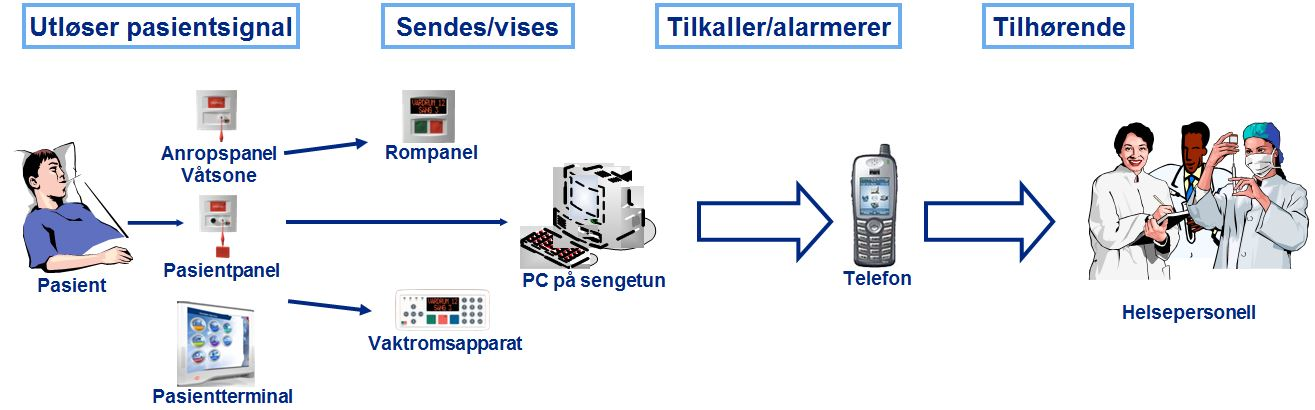
\includegraphics[scale=0.5]{alarmprosess.jpg}
\caption{Dette skjer ved utløst pasientsignal.}
\label{fig:detteskjer}
\end{figure}

\noindent
Sengepostene deles i sengetun, hvor hvert sengetun normalt har seks til åtte pasientrom. Sengetunet er en fysisk og funksjonell måte å organisere pasientrommene, men det er derimot ikke en organisatorisk enhet, og for å sikre fleksibilitet og effektivitet ligger flere sengetun ved en sengepost etter hverandre i serie, som vist i figur \ref{fig:sengepost}. Systemet kan dermed konfigureres på en slik måte at sykepleiere på et sengetun kan motta pasientsignaler fra andre sengetun \cite{Aslaksen}. Vi har i denne oppgaven valgt å se på hvordan pasientsignalsystemet fungerer og brukes på hvert enkelt sengetun isolert sett, og ikke hvordan det brukes i situasjoner hvor signaler mottas fra andre sengetun.

\begin{figure}[H]
\centering
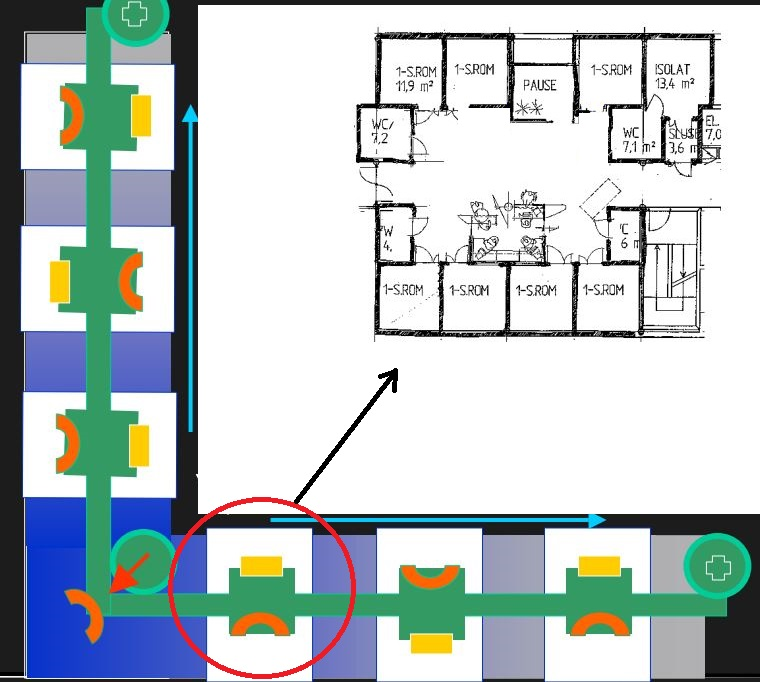
\includegraphics[scale=0.4]{sengepost.jpg}
\caption{Sengepost inndelt i sengetun \cite{Aslaksen}}
\label{fig:sengepost}
\end{figure}

\noindent
Varslingen av sykepleiere, som skjer både via telefon og veggpaneler, gjør sykepleierene utsatt for eksterne avbrytelser i et allerede avbruddsdrevet miljø \cite{Klemets12}. Slike avbrudd i arbeidet kan ha både positive og negative effekter. Avbruddene kan eksempelvis gi informasjon som øker den enkeltes eller gruppens \emph{awareness}, som er nødvendig for koordinert og effektivt arbeid, og som gir bedre beslutningsgrunnlag for hvordan sykepleierene skal håndtere innkommende pasientsignaler. Slik systemet fungerer i dag er avbruddene avgjørende for å formidle denne informasjonen. Likevel vil disse i noen situasjoner være svært forstyrrende, da menneskehjernen kun har begrenset kognitiv kapasitet. Dersom denne overbelastes kan det hemme vedkommendes oppmerksomhet, noe som i verste fall kan føre til livstruende situasjoner. 

\noindent
Ofte vil sykepleiere være involvert i aktiviteter hvor det er problematisk å svare på innkommende pasientsignaler, eksempelvis ved at de er ute til lunsj, befinner seg i isolasjonsrom, eller er hos en pasient de ikke ønsker å forlate. Likevel vil de vises som tilgjengelige i systemet, og dermed motta pasientsignaler som kan oppfattes som forstyrrende. Klemets, Evjemo og Kristiansen (2013) foreslår dermed at videre design av systemet bør tillate sykepleierene å sette seg selv som utilgjengelige. 

\subsubsection{Forskningsspørsmål}
Gjennom arbeidet med denne oppgaven har vi vurdert hvorvidt det er nyttig for sykepleiere å ha informasjon om kollegers aktiviteter og tilgjengelighet, og hvordan slik informasjon kan distribueres på en hensiktsmessig måte. Samtidig ønsket vi å undersøke hvordan systemet kan endres for å redusere eventuelle negative effekter ved avbrytelser. Dette er oppsummert i to forskningsspørsmål:

\begin{enumerate}
\item Er informasjon om kollegers aktiviteter og tilgjengelighet nyttig for sykepleiere, og hvordan kan slik informasjon distribueres på en hensiktsmessig måte? 
\item Hvordan kan systemet endres for å begrense potensielle negative effekter ved avbrytelser?
\end{enumerate}

\noindent
For å besvare disse spørsmålene gjorde vi innledningsvis en gjennomgang av tidligere arbeid og relevant teori. Dette ble utgangspunkt for en prototype som vi testet gjennom workshops, hvor deltagerene fikk vurdere og evaluere fordeler og utfordringer både ved det eksisterende systemet og vår foreslåtte løsning. 

\subsubsection{Avgrensning og disposisjon}
Denne oppgaven er avgrenset til å omhandle sykepleierenes behov til pasientsignalsystemet. Vi har ikke gjort en grundig gjennomgang av underliggende tekniske arkitekturer eller økonomiske aspekter.

\noindent
Oppgaven er strukturert som følger:
\begin{itemize}
\item Kapittel \ref{chp:teori} presenterer relevant teori.
\item Kapittel \ref{chp:forskningsmetode} presenterer hensikten med oppgaven, samt metoder og prosesser vi har benyttet i vårt arbeid. 
\item Kapittel \ref{chp:resultater} oppsummerer de funnene vi har gjort.
\item Kapittel \ref{chp:diskusjon} diskuterer resultatene fra kapittel \ref{chp:resultater}.
\item Kapittel \ref{chp:konklusjon} oppsummerer og konkluderer oppgaven.
\end{itemize}
